% A set X partitioned by a group action into three orbits O_1, O_2, O_3,
% each drawn as a vertical blob of points.
% Source: book/tex/H113/action.tex (§ Orbits and stabilizers).
\documentclass[border=2mm]{standalone}
\usepackage{tikz}
\begin{document}
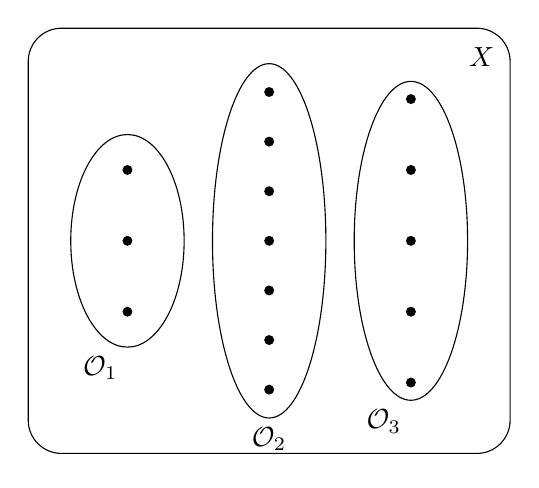
\begin{tikzpicture}[scale=0.9]
  % Ambient set X.
  \draw[rounded corners=12pt] (-3.4,-3) rectangle (3.4,3);
  \node at (3,2.6) {$X$};
  % Three orbits as ellipses.
  \draw (0,0) ellipse (0.8 and 2.5);
  \draw (-2,0) ellipse (0.8 and 1.5);
  \draw (2,0) ellipse (0.8 and 2.25);
  % Points of each orbit.
  \foreach \i in {-3,...,3} \fill (0,0.7*\i) circle (2pt);
  \foreach \p in {(-2,0),(-2,-1),(-2,1)} \fill \p circle (2pt);
  \foreach \p in {(2,0),(2,-1),(2,1),(2,-2),(2,2)} \fill \p circle (2pt);
  % Orbit labels.
  \node[below left] at (-2,-1.5) {$\mathcal O_1$};
  \node[below] at (0,-2.5) {$\mathcal O_2$};
  \node[below left] at (2,-2.25) {$\mathcal O_3$};
\end{tikzpicture}
\end{document}
